\documentclass[a4paper,12pt]{article}
\usepackage{graphicx}
\usepackage[english]{babel}
\usepackage[T1]{fontenc}
\usepackage[utf8]{inputenc}
\usepackage{multirow}
\usepackage{amsmath}
\usepackage{float}
\usepackage{enumerate}
\usepackage{caption}
\usepackage{subcaption}
\usepackage{indentfirst}
\usepackage{color}
\usepackage{array}
\bibliographystyle{unsrt}
\usepackage[top=4cm ,bottom=4cm ,left=3cm ,right=3cm]{geometry}
\usepackage{multirow}
\usepackage{url}

\author{Alex Olar}
\title{CBM simulation}
\date{\today}

\begin{document}
\maketitle
\vfill
\begin{center}
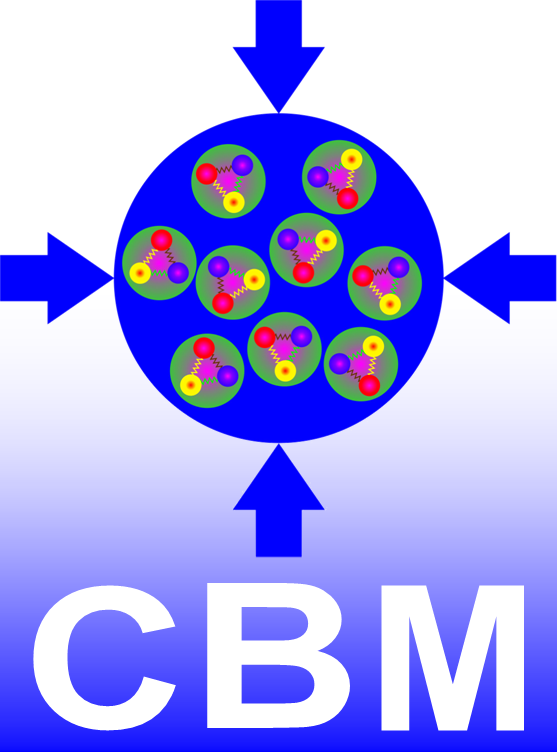
\includegraphics[width=0.66\textwidth]{gsi.png}
\end{center}
\newpage
\renewcommand{\abstractname}{Introduction}
\renewcommand{\thesection}{\Roman{section}.}
\renewcommand{\thesubsection}{\thesection\arabic{subsection}.}
\renewcommand{\thesubsubsection}{\thesubsection\arabic{subsubsection}.}
\begin{abstract}
	\par I have spent one month in summer at the GSI facility, Darmstadt to study the CBM simulation which will be part of FAIR \footnote{ Facility for Antiproton and Ion Research } . During this month I have become experienced with software such as ROOT \footnote{ CERN software for particle physics} , cbmROOT \footnote{ CBM ( Compressed Barionic Matter  ) software for heavy ion physics developped at GSI}, etc.
	\vspace{5mm}
	\par I have learned much about detector technologies and natural phenomena during my stay and I was happy to be part of this huge project and see how scientist work on a daily basis.
\end{abstract}
\tableofcontents
\newpage
\section{Fundamentals}
\subsection{QCD}
\vspace{5mm}
\par In the 20th century physicist realized that symmetries play a crucial role in further understanding the universe. Symmetries led us to conservation laws, the discovery of anti-particles, quarks and much more. 
\vspace{5mm}
\par When quarks were discovered they brought order to the ever increasing particle zoo, as Niels Bohr referred to it. At first, phsysicist only knew three of the six existing quarks, such as: $\textsl{u}$ (up), $\textsl{d}$ (down), $\textsl{s}$ (strange). The hadrons can be separated into two distinct groups: $\textsl{mesons}$ and $\textsl{baryons}$, containing a quark-antiquark pair and three quarks, respectively. The property that distinguishes the quarks is called $\textsl{flavour}$.
\vspace{5mm}
\par A unique feature of the strong interaction, which is the fundamental intereaction between quarks, is confinement, meaning that quarks do not appear in isolation. The charge of the strong interaction is called colours. Due to confinement it means that an elementary particle has to be colour neutral or usually referred to as ''white''. The fundamental theory describing the strong interaction is called Quantum Chromo Dynamics - QCD.
\vspace{5mm}
\par The elementary particles of the QCD are quarks and antiquarks which interact by gluons which also carry charge. There are eight types of gluons since they must describe every elementary colour transformation. These gluons interact with themselves as well.
\subsection{ CBM physics }
\vspace{5mm}
\par When dealing with barionic matter the goal is to understand and map the phase diagram and its transitions. To begin with, I should first have to go through basic thermodynamics and its concepts about phases and their transitions.
\vspace{5mm}
\par The phase diagram of water shows the different phases of it according to pressure and temperature. It is well known that there is a triple point where all three forms of water can coexist such as: liquid water,  solid ice, and water vapor. There are distinct lines between these phases denote, along these lines two phase can coexist at the same time but when changing conditions  the substance must undergo a so called first order phase transition. There is also a critical point which is a state from where to phases differ no more, it is called a smooth $\textsl{crossover}$ from one phase to another.
\begin{figure}[H]
\centering
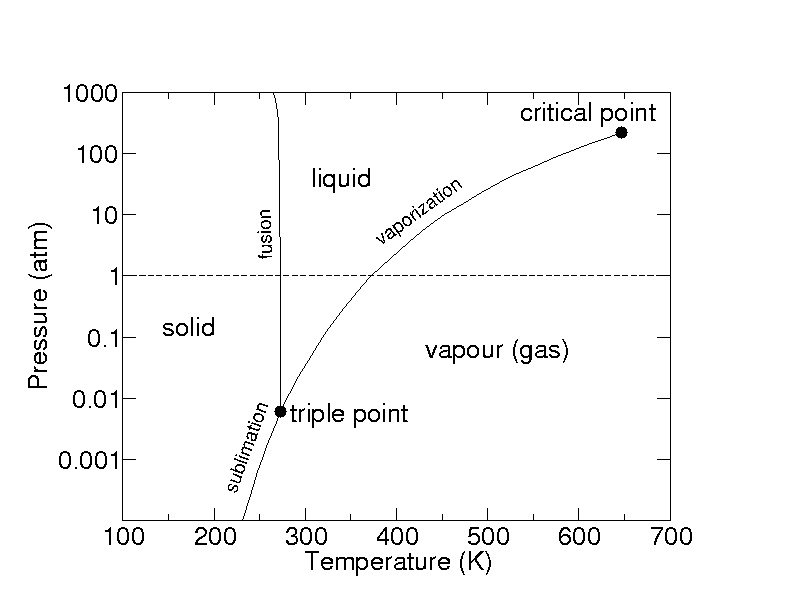
\includegraphics[width=0.66\textwidth]{water_phase.jpg}
\caption{ The previously mentioned phase diagram. }
\end{figure}
\par Now, that I went through the phase diagram of water ( or at least a part of it ) I should move on to matter governed by the strong force. The whole phase diagram of strongly interacting matter is not yet experimentally proved, purely theoretical. It depicts very different and vital phases for being able to describe the early universe or the interior of neutron stars. Each point is described by density and temperature.
 \begin{figure}[H]
\centering
\begin{subfigure}{.49\textwidth}
\centering
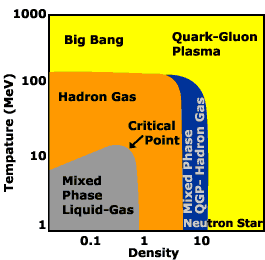
\includegraphics[width=0.92\textwidth]{cbm_phase1.png}
\caption{ Temperature in MeV and densities in units of nuclear bulk density, both scales are logarithmical }
\end{subfigure}
\begin{subfigure}{.49\textwidth}
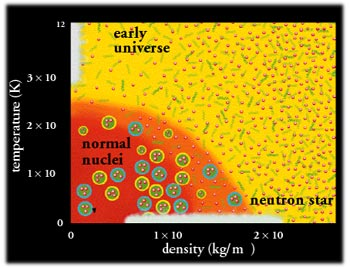
\includegraphics[width=.92\textwidth]{cbm_phase2.jpg}
\caption{ The same diagram that shows why each phase can be crucial to explore further.  }
\end{subfigure}
\end{figure}
 \par As presented above a phase called quark-gluon plasma was present at the Big Bang and later on ceased to exist when temperature dropped. It can be seen that the interior of neutron stars supposedly contains quark-gluon plasma as well as the density is high enough to enalbe matter to exist in that phase altough the very low temperature. 
\vspace{5mm}
\par Obviously the only way to investigate strongly interacting matter on Earth is via high energy particle collisions. It is a characteristic feature of QCD that the coupling between quarks
\end{document}
